\chapter{Problem Description and Approach}\label{chap:chap3}

\section*{}

As described in the section \ref{sec:goals} of the introduction, the project encompasses the creation of a functional prototype for an \emph{Android} mobile application for a platform that uses dynamic social networks and intends to use gamification techniques to improve user engagement. The platform is designed to share information about public transport between travellers.
Before the implementation of the functional prototype, the creation and testing of interface designs is required. 
The usability and interaction of that interface is fundamental to the platform, because it might make the difference between its success or failure, given that it might attract or repel several users and facilitate or make more difficult the submission of information through the platform.

According to a study performed by Robert Pessagno \cite{kn:Pes10}, "[social networks] acceptance is determined by how easy it is to use them", and that has even more importance in the scope of this project, given the necessity of having a large base of users feeding the platform with a huge volume of information in real time at any given moment. If that does not happen, there is a risk of having lines with no information. For instance, low transport frequency time periods or low frequency lines may lead to inexistent information in those lines or during those periods. Having a greater user base mitigates that risk, though it can still happen.

Given the innovation introduced by the main feature of the project, the dynamic social networks, it is necessary to develop suitable metaphors and create user visual affordance to enable the understanding of that feature by travellers, in a familiar or intuitive way for them.
In the first iteration of the project \cite{kn:eSG12}, usability tests were performed in order to capture possible usability problems with the previously developed interface (Figure \ref{fig:current}). 
Those tests resulted in a set of conclusions that encompassed  usability issues to be addressed and aspects to improve in this new iteration, and it is aimed to use those conclusions as a starting point to this work (see \ref{sec:initial}). 

\begin{figure}[h]
\begin{center}
\leavevmode
\subfloat[\emph{Trip information feature.}]{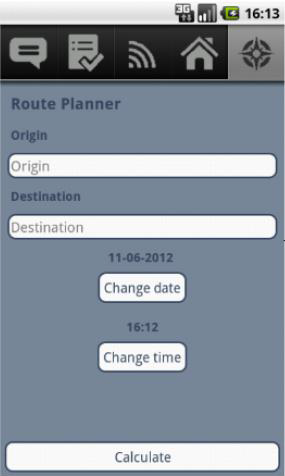
\includegraphics[width=1.7in]{current1.png}} \hspace{1em}%
\subfloat[\emph{Report information feature.}]{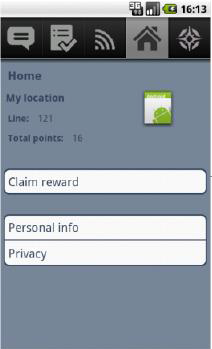
\includegraphics[width=1.7in]{current2.png}}
\subfloat[\emph{Trip information feature.}]{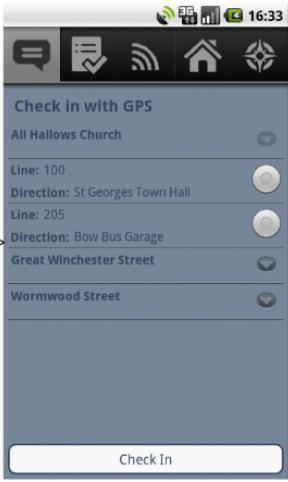
\includegraphics[width=1.7in]{current3.png}}
\caption{Screenshots of the previously implemented interface.}

\label{fig:current}
\end{center}
\end{figure}

\pagebreak

\section{Usability}

Usability can be defined as a measurement for how easy it is to use an interface. Typically, the evaluation or measurement of usability is kept separate from discussions of utility, a characteristic often more influenced by what the interface is connected to (if we're talking about a mobile application, that can be for instance an existing API retrieving data existing in an external server) than the interface itself. 
Jakob Nielsen, one of the most prominent authors and experts on usability, defines usability as having the following components \cite{kn:Nie12}

\begin{itemize}
\item \textbf{Learnability} - How easy it is to users to accomplish basic tasks in the first time they are introduced to the design?
\item \textbf{Efficiency} - Once the users have passed the learning phase, how quickly can they perform tasks?
\item \textbf{Memorability} - After a period of not using the interface, how quickly can users remember it and be proficient in the accomplishment of tasks?
\item \textbf{Errors} - How many errors do the users make while using the interface? What is the severity of those errors and can they recover from them?
\item \textbf{Satisfaction} - How pleasant is it to use the design?
\end{itemize}

Following Nielsen's approach, only actual performance by users is worth measuring. However, there are other approaches, for instance the one defined by Patrick Jordan, that include the theoretical performance level achieved when the system being measured is used to its full potential \cite{kn:Jor94}.

Despite the several definitions and approaches, the goal of  (improving) usability, that aims to be accomplished in this thesis work, is to make it faster and easier to users of an interface to achieve their goals and accomplish the desired tasks.


\section{User-Centered Design}

In the recent years, the attempt of several institutions to integrate design with technology has become a regular behaviour in the development of their products.
In 1999, it was established an international standard, \emph{ISO 13407}, that aimed to provide "guidance on achieving quality in use by incorporating user-centered design activities throughout the life cycle of interactive computer-based systems."

That standard established four activities that had to be started at the earlier stages of a project:

\begin{itemize}
\item Understand and specify the context of use for the product - Collect relevant contextual information from the environment where the system is going to be used;
\item Specify the user and organisational requirements - Formulate and build the user-centered
requirements for the new software.
\item Produce design solutions - Simulate design solutions using paper or computer-based mockups and get feedback of real users;
\item Evaluate designs against requirements. Last but not least,is indispensable to evaluate
the design work performed previously. In this phase anomalies, defects, bugs, failures are detected in order to select the best solution for the system.
\end{itemize}

These activities were meant to be performed according to the workflow presented in Figure \ref{fig:iso}. This standard has since then been revised and re-issued as \emph{ISO 9241-210}, which describes six key principles to apply in a user-centered design process \cite{kn:Tra11}:

\begin{figure}[h!]
  \begin{center}
    \leavevmode
    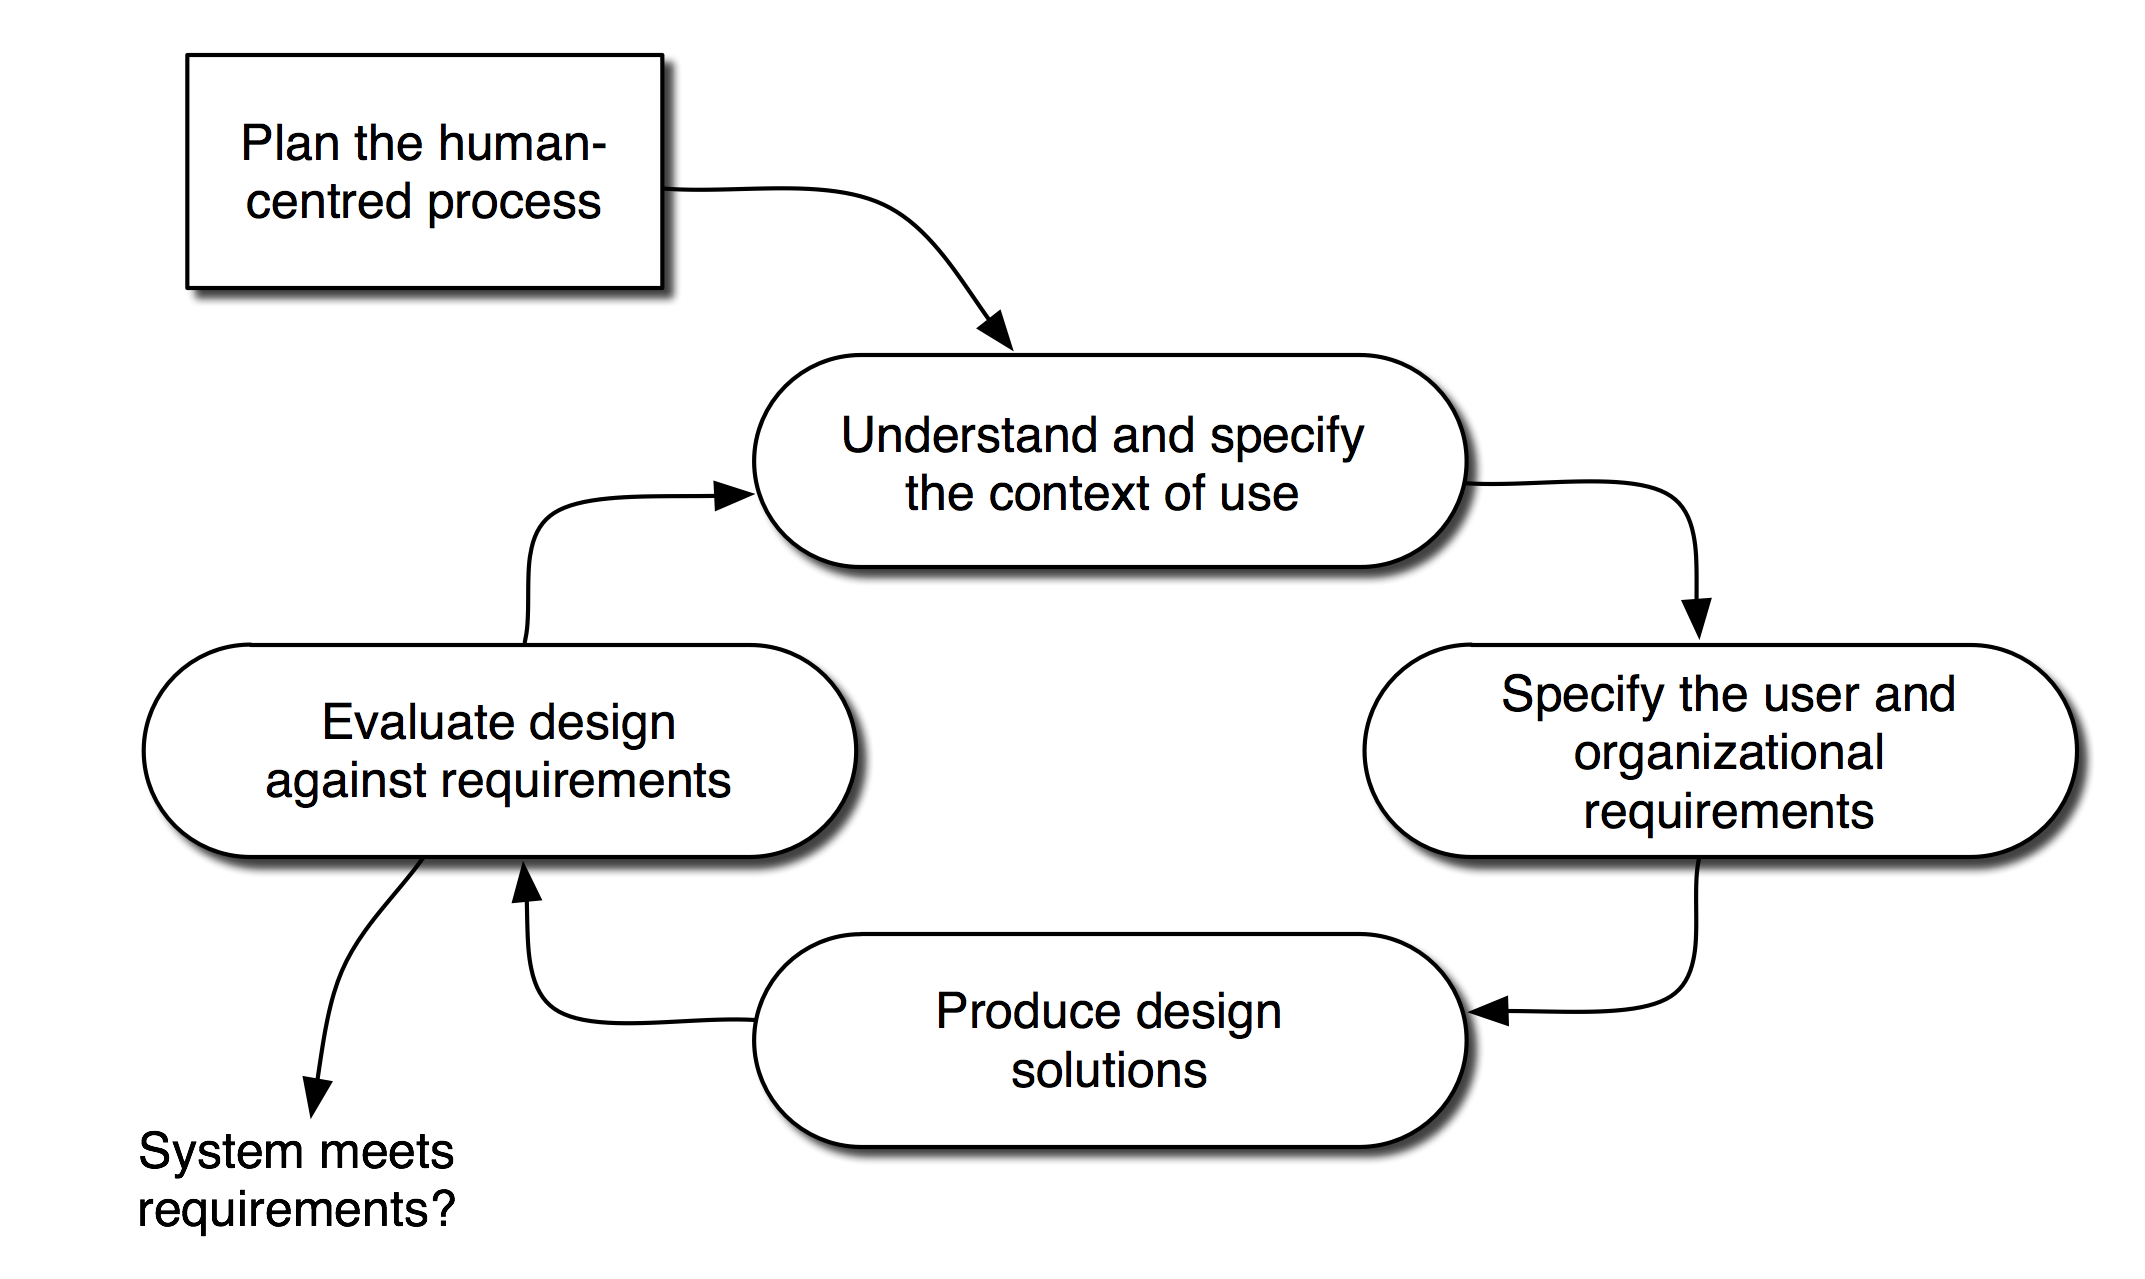
\includegraphics[scale=0.8]{iso13407.png}
    \caption{Workflow of the process described in \emph{ISO 13407}.}
    \label{fig:iso}
  \end{center}
\end{figure}

\begin{itemize}
\item The design is based upon an explicit understanding of users, tasks and environments. This means that is necessary to understand your users, understand what they want to do with the system and understand the environment in which the system is used.

\item Users are involved throughout design and development - Users must be involved in all design phases, not just at the start and at the end of the design.

\item The design is driven and refined by user-centered evaluation - Usability testing should be carried out throughout the design process. Initially, to test preliminary designs such as paper prototypes, and after that, not just at the end of the process.

\item The process is iterative - It is difficult, if not impossible, for users to explain what they want or need from a system. So, in order to find out what people want, it is necessary to show them something that they probably don't want (first designs) and then discover how to improve it. This means that if a waterfall methodology is used the design process will struggle to be user-centered.

\item The design addresses the whole user experience - Usability (and a good user experience) is about a lot more than making things simple, including the perceptual and emotional aspects typically associated with user experience.

\item The design team includes multidisciplinary skills and perspectives - The design team should include a range of views, including the voices of accessibility experts, end users, domain experts, etc.
\end{itemize}



Given those recommendations and the referred importance of making the users part of the development process (thus increasing the chance of success of the application among a wider audience), the chosen process in order to achieve the expected results has four phases: 

\begin{itemize}
\item \textbf{Requirements Elicitation phase} - As an initial step, it should include an analysis of what went wrong or what were the perceived disadvantages in the interface previously conceived, followed by additional usability requirements elicitation (assembling a focus group with potential users of the application and regular public transport users);
\item \textbf{Design phase} - Consists in the creation of alternative low-level designs, along with the usability tests and studies in order to maximize their quality and relevance.
\item \textbf{Prototyping phase} - Implementation of a chosen design, previously done, as an \emph{Android} mobile application.
\item \textbf{Evaluation phase} - Realization of usability evaluation and analysis of the evaluation results, as the name suggests.
\end{itemize}

It is worth referring that this process is an adaptation encompassing the iterative process described in \emph{ISO 13407}, where the mentioned Requirements Elicitation phase serves as the first iteration that allows the gathering of a vast amount of information regarding usability requirements, that will result in the production of an initial design, that will be checked against additional requirements.

The following design phase will act as several iterations of the process, constantly evolving the interface and trying to improve the quality of the solution. That phase will end with a usability test with potential users, that will serve as validation of the evolved design in order to pass to the implementation phase.

Finally, the implementation and evaluation phases will act as a final (and long duration, due to the duration of the implementation) iteration of the process. 

\subsection{Usability Evaluation}

The usual approaches to perform usability evaluation are the following:

\begin{enumerate}
\item \textbf{Usability testing} - Involves measuring typical user's performance on task accomplishment.
\item \textbf{Field studies} - Performed in a natural environment (real case scenario)
\item \textbf{Analytical evaluation} - Does not involve end-users. Two main methods are usually used, heuristic evaluation and/or predictive evaluation. While heuristic evaluation involves the use heuristics (sets of guidelines and standards) and walkthroughs with experts through scenarios of the application prototypes, predictive evaluation is based on theoretical models, in order to predict user performance.
\end{enumerate}

In this project, usability testing, through potential user observation and questioning, will be employed during the development process (as a tool to help with the validation of the interface), while heuristic evaluation with experts will be employed in a final phase, to evaluate the functional prototype and serve as validation of the implemented interface and serve as a base to possible future improvements.

\subsection{Usability Studies}

In order to measure and improve usability of a given project, usability studies are often performed. A usability study serves as an important tool for the evaluation of an User Interface, in which the effectiveness of the User Interface itself is analysed. Based on the results of that evaluation, changes can be made to improve the interface and the interaction of the said project.

These studies often consist in observing users accomplishing a given set of tasks in the application, or even looking at a User Interface and checking it against common design rules and guidelines \cite{kn:Joh14} and identifying the origin of possible unexpected/unwanted behaviours in its utilization. 

In the scope of this project, usability studies will be performed through the design phase, promoting the correction and improvement of the designed interface and crossing those studies with the results of performed usability tests.








